
\subsection[Dielectric materials]{Dielectric materials}
\begin{frame}
  \frametitle{Dielectric materials (I)}

  Tantalum oxynitrides are a class of dielectric materials with high
  $K$ which is tunable by selection of the A cation.  By mixing A
  cations, a temperature-constant dielectric is possible.
  \begin{columns}
    \begin{column}{0.5\linewidth}
      \begin{center}
        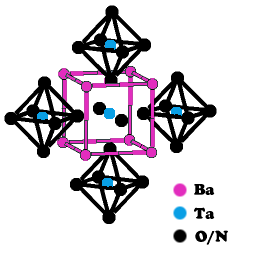
\includegraphics[width=0.6\linewidth]{xas/perovskite.png}
      \end{center}
    \end{column}
    \begin{column}{0.5\linewidth}
      \begin{center}
        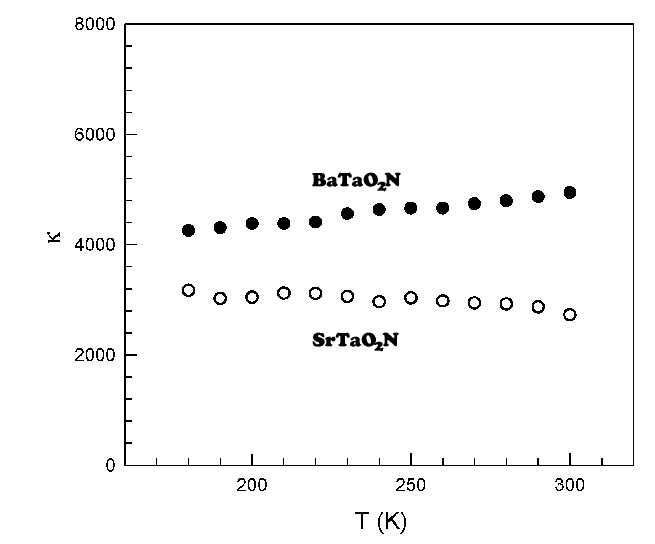
\includegraphics[width=0.9\linewidth]{xas/bton_permit.png}
      \end{center}
    \end{column}
  \end{columns}

  First principles DFT suggests that the different ionic radii of O
  and N introduce substantial disorder around the Ta atom.
  
  \begin{bottomnote}[0.5][19]
    B. Ravel et el., \textit{Role of local disorder in the dielectric
      response of BaTaO$_2$N}, Phys. Rev. \textbf{B73}, p. 184121 (2006),
    \doiref{10.1103/PhysRevB.73.184121}[LightBlue4]
  \end{bottomnote}
\end{frame}

\begin{frame}
  \frametitle{Dielectric materials (II)}%
  The DFT results in a rather complex coordination environment about
  the Ta atom | much more complex than the simple perovskite
  structure.
  \begin{columns}
    \begin{column}{0.5\linewidth}
      \begin{center}
        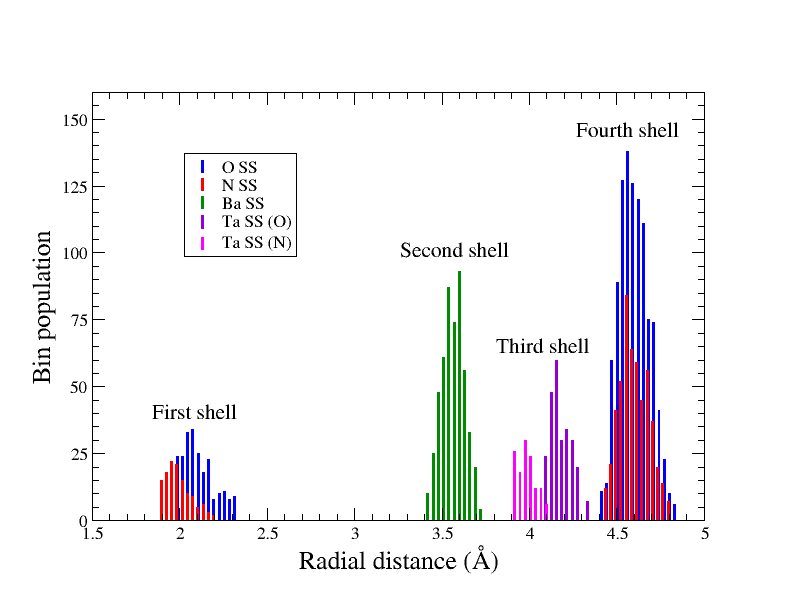
\includegraphics[width=\linewidth]{xas/bton_SS.png}
      \end{center}
    \end{column}
    \begin{column}{0.5\linewidth}
      \begin{center}
        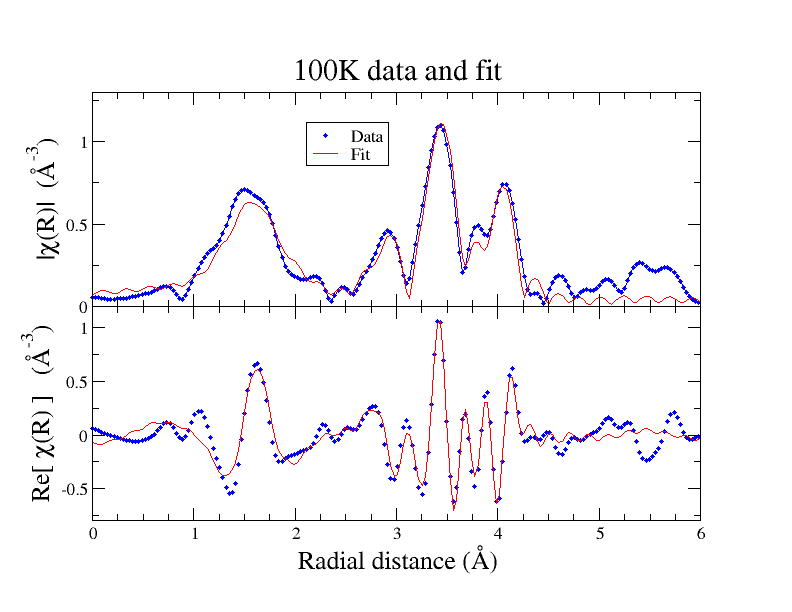
\includegraphics[width=\linewidth]{xas/bton_fit.png}
      \end{center}
    \end{column}
  \end{columns}
  With some effort, this complexity can be incorporated into the data
  analysis.  The EXAFS data are shown to be (mostly) consistent with
  the DFT results.

  \begin{bottomnote}[0.5][19]
    B. Ravel et el., \textit{Role of local disorder in the dielectric
      response of BaTaO$_2$N}, Phys. Rev. \textbf{B73}, p. 184121 (2006),
    \doiref{10.1103/PhysRevB.73.184121}[LightBlue4]
  \end{bottomnote}
\end{frame}
